\documentclass{article}

\def\coq{\textsc{Coq}}
\def\mathcomp{\textsc{MathComp}}
\def\mathcomptwo{\mathcomp~2}
\def\hb{\textsc{HB}}
\def\compdecmodal{\textsc{CompDecModal}}

\usepackage[usenames]{xcolor}
\usepackage{minted}
\setminted{fontsize=\small}
\usemintedstyle{ssr}
\def\coqin#1{\mintinline{ssr}{#1}}

\newminted[failure]{ssr}{bgcolor=lightgray}
\newminted[success]{ssr}{frame=single}

\def\rei#1{{\color{red}{TODO(rei): #1}}}
\def\newterm#1{{\sl #1}}

\usepackage{fullpage}
\usepackage{hyperref}
\usepackage{graphicx}
\usepackage{authblk}

\title{Porting Coq Scripts to \\ the Mathematical Components Library Version 2}
\author[2]{Reynald Affeldt}
\author[1,4]{Yves Bertot}
\author[1,4]{Cyril Cohen}
\author[3]{Pierre Roux}
\author[1]{Kazuhiko Sakaguchi}
\author[1,4]{Enrico Tassi}
\affil[1]{Inria, France}
\affil[2]{National Institute of Advanced Industrial Science and Technology (AIST), Japan}
\affil[3]{ONERA / DTIS, Universit\'e de Toulouse, France}
\affil[4]{Universit\'e C\^ote d'Azur, France}
\date{}                     %% if you don't need date to appear
\setcounter{Maxaffil}{0}

\begin{document}

\maketitle

\begin{abstract}
The Mathematical Components library (hereafter, \mathcomp{})~\cite{mathcompbook} provides,
among others, a number of mathematical structures organized as
hierarchies. Hierarchy Builder (hereafter, \hb) is an extension of the
\coq{} proof assistant to ease the development of hierarchies of
structures~\cite{cohen2020fscd}. \mathcomptwo{}~\cite{mathcomp2} is the result of the
port of \mathcomp{} to \hb{}~\cite{mathcomp2021coq}.

This document is a technical report whose goal is to explain how to
port \mathcomp{} developments to \mathcomptwo.  It has been written by
the participants of the \mathcomp{} Documentation Sprint that happened
from [2023-05-03] to [2023-05-10].
\end{abstract}

\tableofcontents

\section{Target Audience of this Document}

Based on our experience porting several developments to \mathcomptwo,
we can distinguish three categories of users:
\begin{enumerate}
\item \mathcomp{} users who have not been using the \coqin{Canonical}
  command should not see much difference compared to the past version
  upgrades of \mathcomp{}.
  %
  Some identifiers that are now useless have been removed but this is
  documented in the changelog. For example \coqin{bool_eqType} might
  need to be replaced by \coqin{bool : eqType} or just \coqin{bool}.
  %
  Also, the behavior of some rewritings might have changed, requiring
  explicit patterns. Typically, it might happen that rewriting with
  associativity lemmas requires the user to indicate whether it is
  supposed to happen on the left or the right-hand side of an
  equivalence relation, so that \coqin{rewrite addrA} might need to be
  rewritten \coqin{rewrite [in LHS]addrA} for example. See
  Sect.~\ref{sec:other} for a concrete example.
  %
  For such users, reading this tutorial through the end might not be
  necessary.
\item The target readers are primarily \mathcomp{} users who have been
  instantiating structures using the \coqin{Canonical} command.
\item As for the few users who have been developing their own
  hierarchies of structures, this tutorial might be of little help and
  they rather need to refer to:
  \begin{itemize}
  \item the original paper for an extensive introduction to \hb{} commands~\cite{cohen2020fscd},
  \item the \hb{} development for documentation and examples~\cite{hb}
    (start with the \href{https://github.com/math-comp/hierarchy-builder#readme}{README}),
  \item various papers for more applications~\cite{mathcomp2021coq}
    \cite[Sect.~3]{affeldt2022arxiv} \cite[Sect.~4]{affeldt2023cpp},
  \item already ported developments such as
    \href{https://github.com/math-comp/odd-order}{odd-order},
    \href{https://github.com/math-comp/multinomials}{multinomials}, etc.
  \end{itemize}
\end{enumerate}

For the sake of concreteness, we illustrate the port of
\compdecmodal~\cite{compdecmodal} in Sect.~\ref{sec:compdecmodal}.
Before that we review the basics of \hb{} in Sect.~\ref{sec:reminder}
and review the documentation tools available for porting in
Sect.~\ref{sec:explore}.

\section{Quick Reminder about the \hb{} Vocabulary}
\label{sec:reminder}

The goal of this section is to briefly explain the three main commands
introduced by \hb: \coqin{HB.mixin}, \coqin{HB.structure}, and
\coqin{HB.instance}. The knowledgeable reader can safely skip this
section.

Let us consider the most basic scenario in generic terms.  Here is the
pattern to declare a structure \coqin{Struct} that sits at the bottom
of a hierarchy.  The interface of the structure goes into a mixin:
\begin{minted}{ssr}
HB.mixin Record isStruct params carrier := {
  ... properties about the carrier ...
}
\end{minted}

The structure itself is declared like a sigma-type:
\begin{minted}{ssr}
#[short(type=structType)]
HB.structure Definition Struct := {carrier of isStruct carrier}
\end{minted}
Note that \hb{} is using \coq{} attributes to declare the type corresponding to a structure.

Here is the pattern to declare a new structure \coqin{NewStruct} that
extends the existing structure \coqin{Struct}; note the \coqin{of} syntax.
\begin{minted}{ssr}
HB.mixin Record NewStruct_from_Struct params carrier
    of Struct params carrier := {
  ... more properties about the carrier ...
}
\end{minted}

In the case of the extended structure, the sigma-type makes appear the
dependency to the parent structure; note the \coqin{&} syntax.
\begin{minted}{ssr}
#[short(type=newStructType)]
HB.structure NewStruct params :=
  {carrier of NewStruct_from_Struct parames carrier
            & Struct params carrier}.
\end{minted}

This process results in the creation of the types \coqin{structType}
and \coqin{newStructType} such that elements of the latter are also
understood to be elements of the former.

Finally, the declaration of a mixin \coqin{Struct} is accompanied by
the creation of a constructor \coqin{Struct.Build} which is used to instantiate
a structure using the command:
\begin{minted}{ssr}
HB.instance Definition _ := Struct.Build params.
\end{minted}
The command \coqin{HB.instance} should trigger the printing of several
lines of information output such as
\begin{minted}{ssr}
module_type__canonical__struct_Struct is defined
\end{minted}
The absence of this output often indicates failure of the
\coqin{HB.instance} command.

\section{Tools to Port \mathcomp{} Applications}
\label{sec:explore}

\subsection{Documentation}

The following pieces of documentation are useful during the process of
porting a \mathcomp{} application to \mathcomptwo:
\begin{itemize}
\item The changelog is the primary source of information. See \coqin{CHANGELOG.md}~\cite{mathcomp2}.
\item Additionally, structures are documented in the headers of \coq{} scripts
  according to the following format:
\begin{minted}{text}
(*****************************************************************************)
(*                             Centered Title                                *)
(*                                                                           *)
(* Some introductory text: what is this file about, instructions to use this *)
(* file, etc.                                                                *)
(*                                                                           *)
(* Reference: bib entry if any                                               *)
(*                                                                           *)
(* * Section Name                                                            *)
(*   definition == prose explanation of the definition and its parameters    *)
(*     notation == prose explanation, scope information should appear nearby *)
(*   structType == name of structures should make clear the corresponding    *)
(*                 HB structure with the following sentence:                 *) 
(*                 "The HB class is Xyz."                                    *)
(*     shortcut := a shortcut can be explained with (pseudo-)code instead of *)
(*                 prose                                                     *)
(*                                                                           *)
(* Acknowledgments: people                                                   *)
(*****************************************************************************)    
\end{minted}
See for example the \coqin{eqType} structure defined in the file
\coqin{ssreflect/eqtype.v}.
%
See this
\href{https://github.com/math-comp/math-comp/wiki/How-to-document}{wiki
  entry} for more information about the documentation of scripts.
\item Optionally, the user can double-check the naming of identifiers
  and lemmas with the naming conventions explained in
  \coqin{CONTRIBUTING.md}~\cite{mathcomp2}.
\end{itemize}

\subsection{\hb{} Commands Useful to Explore an Existing Hierarchy}

Besides the changelog and the headers of \coq{} scripts, the user can use
\hb{} commands to explore a hierarchy of mathematical structures.

\subsubsection{Information about Structures with \coqin{HB.about}}
\label{sec:info_structures}

Basic information about structures can be obtained via the command
\coqin{HB.about} as in:
\begin{minted}{ssr}
> HB.about eqType.
HB: eqType is a structure (from "./ssreflect/eqtype.v", line 137)
HB: eqType characterizing operations and axioms are:
    - eqP
    - eq_op
HB: eqtype.Equality is a factory for the following mixins:
    - hasDecEq (* new, not from inheritance *)
HB: eqtype.Equality inherits from:
HB: eqtype.Equality is inherited by:
    - SubEquality
    - choice.Choice
...
\end{minted}
(The output message refers to a \newterm{factory}: this is a
generalization of mixin.)

\paragraph{Graph of an \hb{} Hierarchy}

It is also possible to explore a \hb{} hierarchy using the command
\coqin{HB.graph}. Inside a \coq{} file:
\begin{minted}{ssr}
HB.graph "hierarchy.dot".
\end{minted}
From a terminal:
\begin{minted}{text}
tred hierarchy.dot | dot -Tpng > hierarchy.png
\end{minted}
For example, Fig.~\ref{fig:eqtype_hier} displays the immediate
vicinity of \coqin{eqType}.

\begin{figure}[htbp]
\centering
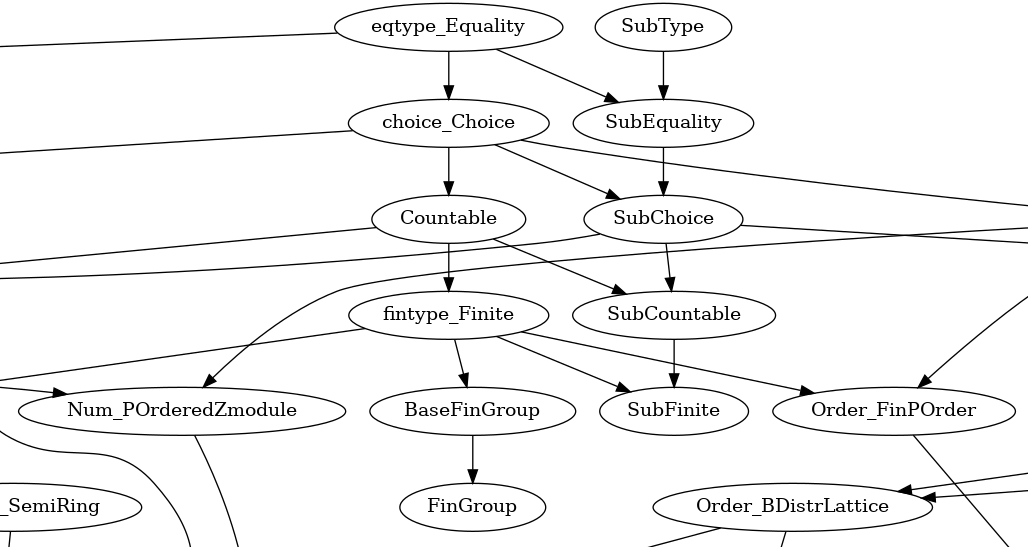
\includegraphics[width=9cm]{eqtype_hier.png}
\caption{The vicinity of the structure {\tt eqType} in \mathcomp{}}
\label{fig:eqtype_hier}
\end{figure}

\subsubsection{Information about Constructors with \coqin{HB.howto} and \coqin{HB.about}}
\label{sec:info_constructors}

To discover constructors that build a structure, one can use the command
\coqin{HB.howto}. For instance
\begin{minted}{ssr}
> HB.howto eqType.
HB: solutions (use 'HB.about F.Build' to see the arguments of each factory F):
    - hasDecEq
\end{minted}
tells us that \coqin{eqType} instances can be built with \coqin{hasDecEq.Build}.
(Note that by default \coqin{HB.howto} may not return all the available factories;
it might be necessary to increase the depth search using a natural number
as in \coqin{HB.howto xyzType 5}.)

To learn which parameters a \coqin{xyz.Build} constructor is expecting, one
can use the \coqin{HB.about} command:
\begin{minted}{ssr}
> HB.about hasDecEq.Build.
HB: hasDecEq.Build is a factory constructor
    (from "./ssreflect/eqtype.v", line 135)
HB: hasDecEq.Build requires its subject to be already equipped with:
HB: hasDecEq.Build provides the following mixins:
    - hasDecEq
HB: arguments: hasDecEq.Build T [eq_op] eqP
    - T : Type
    - eq_op : rel T
    - eqP : Equality.axiom eq_op
\end{minted}
The message indicates that \coqin{hasDecEq.Build} is expecting a type
\coqin{T}, a predicate \coqin{eq_op : rel T} (implicit argument,
as indicated by the square brackets) and a proof of \coqin{Equality.axiom eq_op}.
One can thus instantiate an \coqin{eqType} on some type \coqin{T} with]
\begin{minted}{ssr}
HB.instance Definition _ := hasDecEq.Build T proof_of_Equality_axiom.
\end{minted}
or
\begin{minted}{ssr}
HB.instance Definition _ := @hasDecEq.Build T eq_op proof_of_Equality_axiom.
\end{minted}
which should output a few lines among which (recall that the absence
of this output often indicate an instantiation problem)\footnote{We
  have also observed at the time of this writing that the output of
  the \coqin{HB.instance} command may not be visible by default with
  VSCoq.}:
\begin{minted}{text}
module_T__canonical__eqtype_Equality is defined
\end{minted}

\paragraph{Discover Aliases and Feather Factories}

In addition to the structures and constructors listed by \coqin{HB.about}, the
library defines some aliases (a.k.a.\ feather factories). These aliases
are documented in the header comments. For instance, an \coqin{eqType}
instance on some type \coqin{T} can be derived from some \coqin{T'} already
equipped with an \coqin{eqType} structure, given a function \coqin{f : T -> T'}
and a proof \coqin{injf : injective f}:
\begin{minted}{ssr}
HB.instance Definition _ := Equality.copy T (inj_type injf).
\end{minted}
See \coqin{eqType.v} for \coqin{inj_type}.

\subsubsection{Information about Instances with \coqin{HB.about}}

Instances a type is already equipped with can be listed with
\coqin{HB.about}, for instance:
\begin{minted}{ssr}
> HB.about bool.
HB: bool is canonically equipped with structures:
    - Order.BDistrLattice
      Order.BLattice
      Order.BPOrder
      (from "./ssreflect/order.v", line 6064)
...
\end{minted}
lists all the structures \coqin{bool} is already equipped with.

\section{Porting a \mathcomp{} Development to \mathcomptwo}
\label{sec:compdecmodal}

The basic strategy to port an existing \mathcomp{} development to
\mathcomptwo{} is to (1)~install \mathcomptwo, (2)~compile the existing \coq{}
scripts, and (3)~fix the errors one after the other.
%
For the sake of concreteness, we explain the port of
\compdecmodal~\cite{compdecmodal}. This is a development with a
moderate use of \mathcomp{} whose port involves fixing the
instantiation of basic structures that most developments using
\mathcomp{} are likely to use.

In the following, the offending commands appear in a gray areas
\begin{minted}[bgcolor=lightgray]{text}
command incompatible with MathComp 2
\end{minted}
and their fixes are singly famed:
\begin{minted}[frame=single]{text}
MathComp 2 fix for the command above
\end{minted}

\subsection{Import the \hb{} Library}

First thing first, any \coq{} file using \hb{} must start with:
\begin{minted}{ssr}
From HB Require Import structures.
\end{minted}

\subsection{Instantiation of Structures with \mathcomptwo}

From the viewpoint of the \mathcomp{} user, the main change is the way
mathematical structures are now instantiated. Most \coqin{Canonical}
(or \coqin{Canonical Structure}) commands are replaced by
\coqin{HB.instance} (see Sect.~\ref{sec:reminder}) and there are small
changes to \mathcomp{} notations such \coqin{[subType ...]}, etc.

Regarding \compdecmodal, the first offending set of commands is the
following (file \coqin{fset.v}):
\begin{failure}
Section FinSets.
 Variable T : choiceType.
 ...
 Canonical Structure fset_subType := [subType for elements by fset_type_rect].
 Canonical Structure fset_eqType := EqType _ [eqMixin of fset_type by <:].
 Canonical Structure fset_predType := PredType (fun (X : fset_type) x => nosimpl x \in elements X).
 Canonical Structure fset_choiceType := Eval hnf in ChoiceType _ [choiceMixin of fset_type by <:].
End FinSets.

Canonical Structure fset_countType (T : countType) :=
  Eval hnf in CountType _ [countMixin of fset_type T by <:].
Canonical Structure fset_subCountType (T : countType) :=
  Eval hnf in [subCountType of fset_type T].
\end{failure}

Let us consider compilation errors in order:
\begin{failure}
> Canonical Structure fset_subType := [subType for elements by fset_type_rect].
Error: Syntax error: [reduce] expected after ':=' (in [def_body]).
\end{failure}
This error is due to a change of notation that is documented in the
changelog.  Search for the string, say, ``\coqin{[subType}'' in
\coqin{CHANGELOG.md}:
\begin{minted}{text}
- in `eqtype.v`
  ...
  + notation `[subType for v by rec]`, use `[isSub for v by rec]`
  ...
\end{minted}
The fix is therefore the following:
\begin{success}
> HB.instance Definition _ := [isSub for elements by fset_type_rect].
HB_unnamed_factory_3 is defined
fset_fset_type__canonical__eqtype_SubType is defined
\end{success}
Note that the instance need not be named and better not be since it is
the job of \hb{} to figure out instances automatically.
%
It is important to check that \hb{} displays more than one message as
a response to \coqin{HB.instance}, otherwise this might indicate a
failed instantiation.

Next compilation error:
\begin{failure}
> Canonical Structure fset_eqType := EqType _ [eqMixin of fset_type by <:].
Error: The reference EqType was not found in the current environment.
\end{failure}
This error is primarily due to the remove of the \coqin{EqType}
constructor~\cite[Sect.~2.1]{garillot2009tphols}. In fact, most
\coqin{xyzType} constructors from \mathcomp{} should not be necessary
anymore. See the changelog.
%
Similarly to the \coqin{[subType for _ by _]} notation above, 
the \coqin{[eqMixin of _ by <:]} has changed:
\begin{minted}{text}
- in `eqtype.v`
  ...
  + notation `[eqMixin of T by <:]`, use `[Equality of T by <:]`
  ...
\end{minted}
The fix is therefore:
\begin{success}
> HB.instance Definition _ := [Equality of fset_type by <:].
HB_unnamed_factory_8 is defined
eqtype_Equality__to__eqtype_hasDecEq is defined
HB_unnamed_mixin_10 is defined
fset_fset_type__canonical__eqtype_Equality is defined
fset_fset_type__canonical__eqtype_SubEquality is defined
\end{success}

The next two compilation errors are similarly due to the removal of
\coqin{choiceType} and \coqin{CountType}, and to the change of the
notations \coqin{[choiceMixin of _ by <:]} and \coqin{[countMixin of _
  by <:]}:
\begin{failure}
> Canonical Structure fset_choiceType := Eval hnf in ChoiceType _ [choiceMixin of fset_type by <:].
Error: The reference ChoiceType was not found in the current environment.
> Canonical Structure fset_countType (T : countType) :=
>   Eval hnf in CountType _ [countMixin of fset_type T by <:].
Error: The reference CountType was not found in the current environment.
\end{failure}
The fix can again be inferred from the changelog:
\begin{success}
> HB.instance Definition _ := [Choice of fset_type by <:].
HB_unnamed_factory_11 is defined
choice_Choice__to__choice_hasChoice is defined
HB_unnamed_mixin_14 is defined
fset_fset_type__canonical__choice_Choice is defined
fset_fset_type__canonical__choice_SubChoice is defined
> HB.instance Definition _ (T : countType) := [Countable of fset_type T by <:].
T is declared
HB_unnamed_factory_30 is defined
choice_Countable__to__choice_hasChoice is defined
choice_Countable__to__eqtype_hasDecEq is defined
choice_Countable__to__choice_Choice_isCountable is defined
HB_unnamed_mixin_34 is defined
fset_fset_type__canonical__choice_Countable is defined
fset_fset_type__canonical__choice_SubCountable is defined
\end{success}
Note that, although \hb{} does provide an \mintinline{ssr}{#[hnf]} attribute, it
should not be necessary in general.

Finally, the last \coqin{Canonical} command causes a deprecation
warning that needs to be addressed:
\begin{failure}
> Canonical Structure fset_subCountType (T : countType) :=
>  Eval hnf in [subCountType of fset_type T].
Warning: Notation "[ subCountType of _ ]" is deprecated since mathcomp 2.0.0.
Use SubCountable.clone instead.
[deprecated-notation,deprecated]
fset_subCountType is defined  
\end{failure}
In fact, going back one step, it can be observed by the output the
\coqin{HB.instance} commands that the instantiation of the
\coqin{Countable} structure already triggered the instantiation of the
\coqin{SubCountable} structure, rendering the last \coqin{Canonical}
command harmful. It therefore needs to be deleted.

To sum up, here follows the complete fix:
\begin{minted}[frame=single,numbers=left,escapeinside=??]{ssr}
Section FinSets.
 Variable T : choiceType.
 ...
 HB.instance Definition _ := [isSub for elements by fset_type_rect].
 HB.instance Definition _ := [Equality of fset_type by <:]. ?\label{line:eqtype}?
 Canonical Structure fset_predType := PredType (fun (X : fset_type) x => nosimpl x \in elements X).
 HB.instance Definition _ := [Choice of fset_type by <:]. ?\label{line:choicetype}?
End FinSets.

HB.instance Definition _ (T : countType) := [Countable of fset_type T by <:]. ?\label{line:countttype}?
\end{minted}

In fact, we can go one step further. Instead of instantiating the
\coqin{Equality} structure at line~\ref{line:eqtype} and then the
\coqin{Choice} structure at line~\ref{line:choicetype}, one can start
by instantiating the \coqin{Choice} structure and get the
\coqin{Equality} structure automatically, so that a shorter fix would
be:
\begin{success}
Section FinSets.
 Variable T : choiceType.
 ...
 HB.instance Definition _ := [isSub for elements by fset_type_rect].
 HB.instance Definition _ := [Choice of fset_type by <:].
 Canonical Structure fset_predType := PredType (fun (X : fset_type) x => nosimpl x \in elements X).
End FinSets.

HB.instance Definition _ (T : countType) := [Countable of fset_type T by <:].
\end{success}
This small example already illustrates the advantage of porting to \mathcomptwo.

\subsection{Finitely Iterated Operators}

The next series of compilation errors that occur when porting
\compdecmodal{} is about finitely iterated operators, which are likely
to be used by most \mathcomp{} developments:
\begin{failure}
Canonical Structure fsetU_law (T : choiceType) := 
  Monoid.Law (@fsetUA T) (@fset0U T) (@fsetU0 T).
Canonical Structure fsetU_comlaw (T : choiceType) := 
  Monoid.ComLaw (@fsetUC T).
\end{failure}

The first compilation error indicates a change in the signature of a constructor:
\begin{failure}
> Canonical Structure fsetU_law (T : choiceType) := 
>   Monoid.Law (@fsetUA T) (@fset0U T) (@fsetU0 T).
Error:
In environment
T : choiceType
The term "fsetUA (T:=T)" has type "forall X Y Z : {fset T}, X `|` (Y `|` Z) = X `|` Y `|` Z"
while it is expected to have type "Type".
\end{failure}
We can use \coqin{HB.about} to discover the relevant structure (see Sect.~\ref{sec:info_structures}):
\begin{minted}{ssr}
> HB.about Monoid.Law.
HB: Monoid.Law.type is a structure (from "./ssreflect/bigop.v", line 415)
...
\end{minted}
We can now use \coqin{HB.howto} to discover how to build this structure (see Sect.~\ref{sec:info_constructors}):
\begin{minted}{ssr}
> HB.howto Monoid.Law.type
HB: solutions (use 'HB.about F.Build' to see the arguments of each factory F):
    - Monoid.isLaw
    - SemiGroup.isLaw; Monoid.isMonoidLaw
\end{minted}
Finally, we can use \coqin{HB.about} to learn about the parameters of a constructot (see Sect.~\ref{sec:info_constructors}):
\begin{minted}{ssr}
> HB.about Monoid.isLaw.Build
...
HB: arguments: Monoid.isLaw.Build T idm op opA op1m opm1
    - T : Type
    - idm : T
    - op : T -> T -> T
    - opA : associative op
    - op1m : left_id idm op
    - opm1 : right_id idm op
\end{minted}
We have now enough information to fix the compilation error:
\begin{success}
HB.instance Definition _ (T : choiceType) := 
  Monoid.isLaw.Build {fset T} fset0 fsetU (@fsetUA T) (@fset0U T) (@fsetU0 T).  
\end{success}
Note that we have made explicit the \newterm{key} (the operator
\coqin{fsetU}) in the instantiation. Though not strictly necessary, this is
good practice to document it on this occasion.

\bigskip

Next compilation error:
\begin{failure}
> Canonical Structure fsetU_comlaw (T : choiceType) := 
>   Monoid.ComLaw (@fsetUC T).
Error:
In environment
T : choiceType
The term "fsetUC (T:=T)" has type "forall X Y : {fset T}, X `|` Y = Y `|` X"
  while it is expected to have type "Type".  
\end{failure}
This is similar to above: use \coqin{HB.about} to learn about
\coqin{Monoid.ComLaw} and use \coqin{HB.howto} to inquire about its construction.
\begin{minted}{ssr}
> HB.howto Monoid.ComLaw.type.
HB: solutions (use 'HB.about F.Build' to see the arguments of each factory F):
    - Monoid.isComLaw
    - SemiGroup.isComLaw; Monoid.isMonoidLaw
    - SemiGroup.isCommutativeLaw; Monoid.isLaw
    - SemiGroup.isLaw; SemiGroup.isCommutativeLaw; Monoid.isMonoidLaw
\end{minted}
Note that since the key \coqin{fsetU} has already been equipped with a \coqin{Monoid.Law} structure,
we can add this key as an additional parameter to \coqin{HB.howto} to restrict the search:
\begin{minted}{ssr}
> HB.howto fsetU Monoid.ComLaw.type.
HB: solutions (use 'HB.about F.Build' to see the arguments of each factory F):
    - SemiGroup.isCommutativeLaw
\end{minted}
We can then check the parameters of \coqin{SemiGroup.isCommutativeLaw.Build} to come up with the following fix:
\begin{success}
HB.instance Definition _ (T : choiceType) :=
  SemiGroup.isCommutativeLaw.Build _ fsetU (@fsetUC T).
\end{success}

To sum up, we fix the compilation errors about finitely iterated operators using:
\begin{success}
HB.instance Definition _ (T : choiceType) :=
  SemiGroup.isCommutativeLaw.Build _ fsetU (@fsetUC T).
HB.instance Definition _ (T : choiceType) := 
  Monoid.isLaw.Build {fset T} fset0 fsetU (@fsetUA T) (@fset0U T) (@fsetU0 T).  
\end{success}
In fact, we could have proceeded with only one instantiation since
we can get the \coqin{Monoid.Law} structure from the instantiation of the 
\coqin{Monoid.ComLaw} structure, so that a better fix would be:
\begin{success}
HB.instance Definition _ (T : choiceType) :=
  Monoid.isComLaw.Build _ _ fsetU (@fsetUA T) (@fsetUC T) (@fset0U T).
\end{success}

\subsection{Other Compilation Errors}
\label{sec:other}

Since other compilation errors are similar to the one already explained above, we go faster about them.

\paragraph{Instantiation of an \coqin{Equality} Structure}

Next failure in the file \coqin{K/K_def.v}:
\begin{failure}
Definition form_eqMixin := EqMixin (compareP eq_form_dec).
Canonical Structure form_eqType := Eval hnf in @EqType form form_eqMixin.
\end{failure}
The failure is primarily caused by the removal of \coqin{EqMixin}. The changelog
suggests to use the constructor \coqin{hasDecEq.Build} whose parameters
can be double-checked with \coqin{HB.howto} leading to the following fix:
\begin{success}
HB.instance Definition _ := hasDecEq.Build form (compareP eq_form_dec).  
\end{success}

\paragraph{Instantiation of a \coqin{Countable} Structure}

Next failure in the file \coqin{K/K_def.v}:
\begin{failure}
Definition form_countMixin := PcanCountMixin formChoice.pickleP.
Definition form_choiceMixin := CountChoiceMixin form_countMixin.
Canonical Structure form_ChoiceType := Eval hnf in ChoiceType form form_choiceMixin.
Canonical Structure form_CountType := Eval hnf in CountType form form_countMixin.  
\end{failure}
We learn that \coqin{PcanCountMixin} is deprecated and that
\coqin{CountChoiceMixin} is no more. The changelog suggests to use
\coqin{PCanIsCountable} instead of \coqin{PcanCountMixin}.  According
to \coqin{Locate}, \coqin{PCanIsCountable} is located in the file
\coqin{ssreflect/choice.v} and it has the following type:
\begin{minted}{ssr}
PCanIsCountable :
forall [T : countType] [sT : Type] [f : sT -> T] [f' : T -> option sT], pcancel f f' ->
  isCountable.axioms_ sT
\end{minted}
The fix in this case is therefore:
\begin{success}
HB.instance Definition _ : isCountable form := PCanIsCountable formChoice.pickleP.  
\end{success}
Note that we have added a type information to make the key (here,
\coqin{form}) explicit as recommended when performing instantiations.
This fix is sufficient because it generates the \coqin{Choice} instance
along with the \coqin{Countable} instance.

\paragraph{More Instantiations of \coqin{Equality} Structures}

The next compilation errors in the files \coqin{Kstar_def.v}, \coqin{gen_def.v},
and \coqin{CTL_def.v} are handled as already explained above.

\paragraph{Failing Rewriting}

The next compilation ``error'' is in the file \coqin{CTL/demo.v}.
It is actually a tactic whose execution has been substantially slowed down by the upgrade to \mathcomptwo:
\begin{failure}
move => [p' y]. rewrite /MRel /Mstate (negbTE (root_internal _)) [_ && _]/= orbF.
\end{failure}
The offending rewrite is the one with \coqin{orbF}. It used to apply
by default to the left-hand side of an \coqin{<->} equivalence but now
the user is required to indicate the rewrite location with a pattern
to recover a reasonable execution time:
\begin{success}
move => [p' y]. rewrite /MRel /Mstate (negbTE (root_internal _)) [_ && _]/=.
rewrite [in X in X <-> _]orbF.
\end{success}
This kind of slow down is however rather exceptional.

\bigskip

There are a few more compilation errors but they are similar to the ones we explained so far.

\section{Conclusion}

This document illustrated the port of a typical \mathcomp{}
development to \mathcomptwo. We reviewed the available tools
(documentation and \hb{} tactics) and went through a number of
concrete sample errors and warnings that we explained and corrected.

The example of porting \compdecmodal{} demonstrated that the use of
\hb{} improves the \coq{} scripts in terms of readability and even
allows for improvements. The complete fix can be found
\href{https://github.com/affeldt-aist/comp-dec-modal/tree/tutorial_mathcomp2}{online},
it required the edition of 10 files, 35 insertions, and 67 deletions,
which arguably represents a moderate amount of work.

The migration process to \mathcomptwo{} will surely generate more
questions that the community is ready to answer via the math-comp
streams on \url{https://coq.zulipchat.com}.


\bibliographystyle{abbrv}
\bibliography{porting}

\end{document}